\documentclass{template}
\usepackage[table]{xcolor}
\usepackage[T5]{fontenc}
\usepackage[utf8]{inputenc}
\usepackage[vietnamese]{babel}
\usepackage{amsmath}
\usepackage{lipsum}
\definecolor{bg}{rgb}{0.95,0.95,0.95}
\title{}
\usepackage{listings}
\usepackage{multirow}
\usepackage{float}
\usepackage{adjustbox}
\usepackage{graphicx}
\usepackage{colortbl}
\usepackage{hyperref}
\usepackage{url}
\usepackage{xurl}
\usepackage[utf8]{inputenc}
\usepackage{cite}
\usepackage{booktabs}
\usepackage{tabularx}
\usepackage{longtable}
\renewcommand{\bibname}{References}

\lstset{
    language=C++,
    basicstyle=\ttfamily\small,
    keywordstyle=\color{blue},
    commentstyle=\color{green!40!black},
    stringstyle=\color{red},
    showstringspaces=false,
    breaklines=true,
    frame=tb,
    numbers=left,
    numberstyle=\tiny\color{gray},
    stepnumber=1,
    numbersep=5pt,
    backgroundcolor=\color{gray!10},
    tabsize=4,
    captionpos=b,
    columns=fullflexible
}

\begin{document}

\titre{Temporal Robustness in Face Recognition}
\sujet{CS331.Q11.KHTN - Thị giác máy tính nâng cao}

\enseignant{TS. Mai Tiến Dũng}
\eleves{Nguyễn Văn Minh - 23521418 \\
Nguyễn Văn Hồng Thái - 23521418}

\fairemarges
\fairepagedegarde
\tabledematieres

% Import các chapter
\chapter{Thông tin thành viên và Phân công nhiệm vụ}

\section*{1. Nguyễn Văn Hồng Thái}
\begin{itemize}
    \item \textbf{MSSV:} 23521418
    \item \textbf{Email:} 23521418@gm.uit.edu.vn
    \item \textbf{Mức độ hoàn thành:} 100\%
\end{itemize}

\textbf{Nhiệm vụ được phân công:}
\begin{enumerate}
    \item \textbf{Thực nghiệm và tổng hợp báo cáo phần:}
    \begin{itemize}
        \item Lên ý tưởng, đọc và tổng hợp tài liệu tham khảo.
        \item Thông tin thành viên và đánh giá.
        \item Lý do và tầm quan trọng của bài toán (Motivation \& Importance).
        \item Phát biểu bài toán (Problem Statement): Xác định Input/Output.
        \item Dùng hương pháp giải quyết: Mô hình \textbf{ArcFace}.
        \item Chuẩn bị nội dung slide thuyết trình tương ứng.
        \item Tổng hợp tài liệu tham khảo.
    \end{itemize}
\end{enumerate}

\section*{2. Nguyễn Văn Minh}
\begin{itemize}
    \item \textbf{MSSV:} 23520945
    \item \textbf{Email:} 23520945@gm.uit.edu.vn
    \item \textbf{Mức độ hoàn thành:} 100\%
\end{itemize}

\textbf{Nhiệm vụ được phân công:}
\begin{enumerate}
    \item \textbf{Thực nghiệm và báo cáo phần:}
    \begin{itemize}
        \item Lên ý tưởng, đọc và tổng hợp tài liệu tham khảo.
        \item Dùng phương pháp giải quyết: Mô hình \textbf{MagFace}.
        \item Kết quả thực nghiệm (Experimental Results).
        \item Đánh giá, nhận xét ưu điểm và hạn chế (Evaluation).
        \item Chuẩn bị nội dung slide thuyết trình tương ứng.
        \item Tổng hợp tài liệu tham khảo.
    \end{itemize}
\end{enumerate}

\chapter{Giới thiệu}

\section{Lý do chọn đề tài}

\subsection{Thách thức từ sự thay đổi sinh học theo thời gian}
Trong những năm gần đây, các hệ thống nhận diện khuôn mặt (Face Recognition - FR) đã đạt được những bước tiến vượt bậc, hoạt động hiệu quả trong các điều kiện tiêu chuẩn với ảnh chụp gần thời điểm xác thực. Tuy nhiên, hiệu năng của các hệ thống này vẫn gặp phải sự suy giảm đáng kể khi đối mặt với các dữ liệu khuôn mặt thay đổi theo thời gian dài hạn.
\\
Về mặt sinh học, khuôn mặt con người là một thực thể thay đổi liên tục. Quá trình lão hóa làm biến đổi cấu trúc xương, cơ và bề mặt da, dẫn đến sự thay đổi của các đặc trưng thị giác cốt lõi. Đây là một thách thức lớn đối với các thuật toán nhận diện, bởi các đặc trưng này cần phải đủ tính "bất biến" (invariant) để nhận diện chính xác qua nhiều năm. Tuy nhiên, thực tế thường xảy ra hiện tượng "trôi đặc trưng" (feature drift), khiến khoảng cách giữa các vector đặc trưng của cùng một người tăng lên theo thời gian, làm giảm độ chính xác của mô hình.
\begin{figure}[H] 
    \centering
    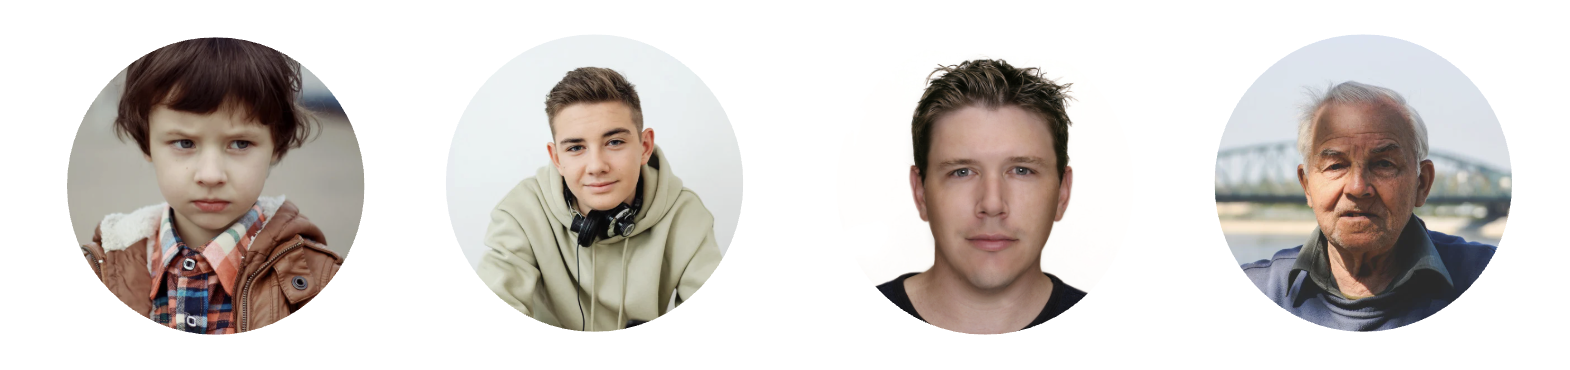
\includegraphics[width=0.8\linewidth]{logos/1.png} 
    \caption{Minh họa sự thay đổi khuôn mặt theo thời gian (Face Aging)} 
\end{figure}

Ngoài ra, sự thiếu hụt các bộ dữ liệu huấn luyện cân bằng, với tỷ lệ ảnh người lớn tuổi thường rất thấp, đặt ra câu hỏi lớn: Liệu sự suy giảm độ chính xác là do giới hạn bản chất của thuật toán hay do sự thiên lệch của dữ liệu? Việc nghiên cứu vấn đề này giúp làm sáng tỏ giới hạn của các mô hình State-of-the-art (SOTA) hiện nay.

\section{Tầm quan trọng của bài toán}

\subsection{Ứng dụng thực tiễn trong An ninh và Xác thực lâu dài}
Tính bền vững theo thời gian (Temporal Robustness) không chỉ là một vấn đề học thuật mà còn là yếu tố sống còn đối với các hệ thống thực tế:
\begin{itemize}
    \item \textbf{Giám sát và An ninh (Surveillance \& Security):} Các hệ thống an ninh cần có khả năng nhận diện các đối tượng truy nã hoặc giám sát ngay cả khi dữ liệu hồ sơ của họ (gallery images) đã được thu thập từ nhiều năm trước.
    \item \textbf{Giấy tờ tùy thân:} Ảnh trên Căn cước công dân (CCCD) hoặc Hộ chiếu (Passport) thường có giá trị sử dụng kéo dài từ 10 đến 20 năm. Các hệ thống e-Gate tại cửa khẩu hoặc xác thực ngân hàng (eKYC) phải xử lý được khoảng cách thời gian lớn (time gap) này mà không gây ra lỗi xác thực sai, đảm bảo trải nghiệm người dùng và an ninh quốc gia.
    \item \textbf{Thiết bị cá nhân:} Với việc mở khóa điện thoại bằng khuôn mặt hàng ngày, hệ thống cần có khả năng "học" và thích nghi với sự lão hóa dần dần của người dùng mà không yêu cầu việc đăng ký lại khuôn mặt liên tục.
\end{itemize}
\begin{figure}[H] 
    \centering
    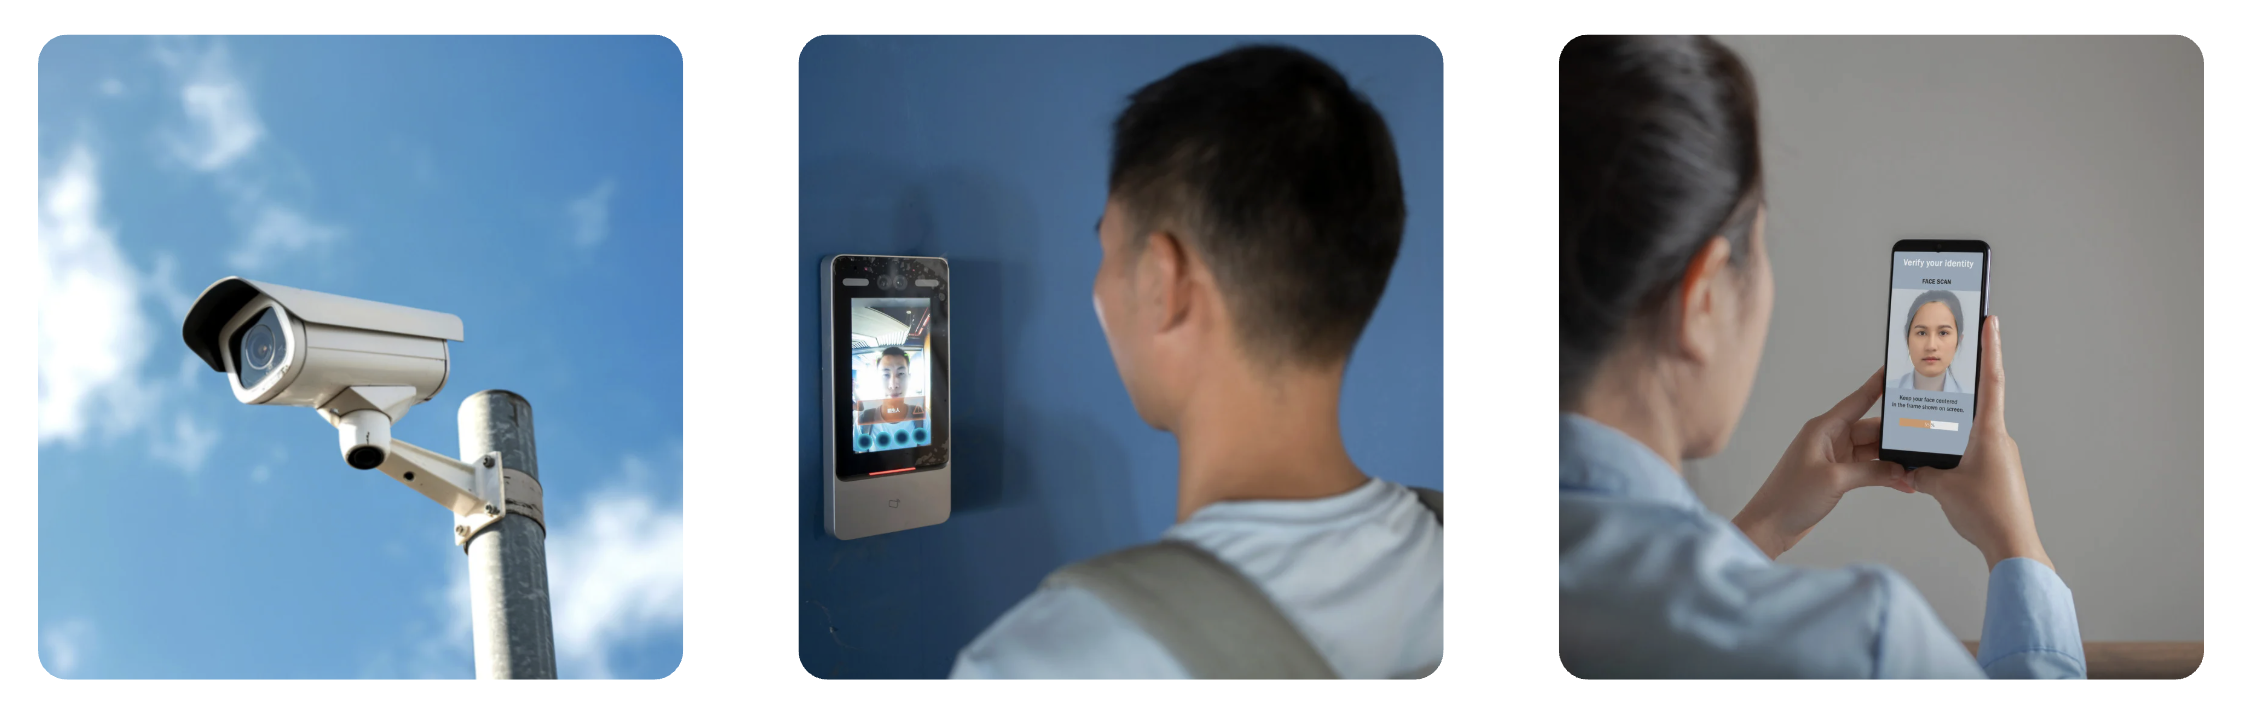
\includegraphics[width=0.8\linewidth]{logos/2.png} 
    \caption{Ứng dụng thực tiễn của nhận diện khuôn mặt bền vững theo thời gian} 
\end{figure}

\subsection{Đóng góp vào việc cải thiện và đánh giá độ tin cậy của thuật toán}
Việc định lượng mức độ suy giảm hiệu năng (degradation rate) của các mô hình tiên tiến như ArcFace hay MagFace theo từng khoảng thời gian (2 năm, 5 năm, 10 năm) mang lại giá trị thực tiễn cao. Nếu hệ thống hoạt động kém trên một nhóm tuổi cụ thể (ví dụ: người cao tuổi), điều này có thể dẫn đến các lỗ hổng bảo mật hoặc sự phân biệt đối xử trong cung cấp dịch vụ số.

Bài toán này tập trung so sánh giữa \textbf{ArcFace} (sử dụng biên góc cố định) và \textbf{MagFace} (sử dụng biên thích ứng dựa trên chất lượng ảnh). Kết quả phân tích các chỉ số như EER hay TAR@FAR sẽ cung cấp cái nhìn sâu sắc (insight) về cách tối ưu hóa hàm loss để xử lý tốt hơn các khuôn mặt có độ tuổi thay đổi, tạo tiền đề cho việc phát triển các mô hình "Age-Invariant" trong tương lai.

\chapter{Phát biểu bài toán}

\section{Mục tiêu nghiên cứu}
Bài toán được thực hiện không chỉ dừng lại ở nhiệm vụ nhận diện khuôn mặt cơ bản mà đi sâu vào đánh giá định lượng (Quantitative Evaluation) hiệu năng của mô hình trước tác động của thời gian. Các mục tiêu cụ thể bao gồm:

\begin{enumerate}
    \item \textbf{Kiểm chứng "Nghịch lý tuổi tác":} Trước đây, các nghiên cứu trên các đặc trưng thủ công (hand-crafted features) thường cho rằng người già dễ nhận diện hơn do cấu trúc khuôn mặt ổn định. Bài toán này tập trung chứng minh thực tế ngược lại đối với các mô hình Deep CNN hiện đại: độ chính xác nhận diện thường thấp hơn ở nhóm người cao tuổi do sự suy giảm chất lượng phân phối giả mạo (impostor distribution).
    
    \item \textbf{Đo lường sự suy giảm hiệu năng (Degradation Rate):} Tính toán và định lượng mức độ giảm sút của độ chính xác nhận diện khi khoảng cách thời gian (Time Gap) giữa hai lần chụp tăng dần (theo các mốc 2, 4, 6, 8, 10 năm).
    
    \item \textbf{So sánh tính bền vững của các hàm Loss:} Đánh giá hiệu quả của cơ chế "Biên thích ứng" (Adaptive Margin) trong MagFace so với cơ chế "Biên cố định" (Fixed Margin) trong ArcFace khi xử lý dữ liệu có độ chênh lệch tuổi tác lớn, từ đó rút ra các nhận định về hướng tối ưu hóa mô hình.
\end{enumerate}

\section{Đặc tả Input và Output}
Để giải quyết các mục tiêu trên, hệ thống thực nghiệm được thiết kế với luồng dữ liệu như sau:
\begin{figure}[H] 
    \centering
    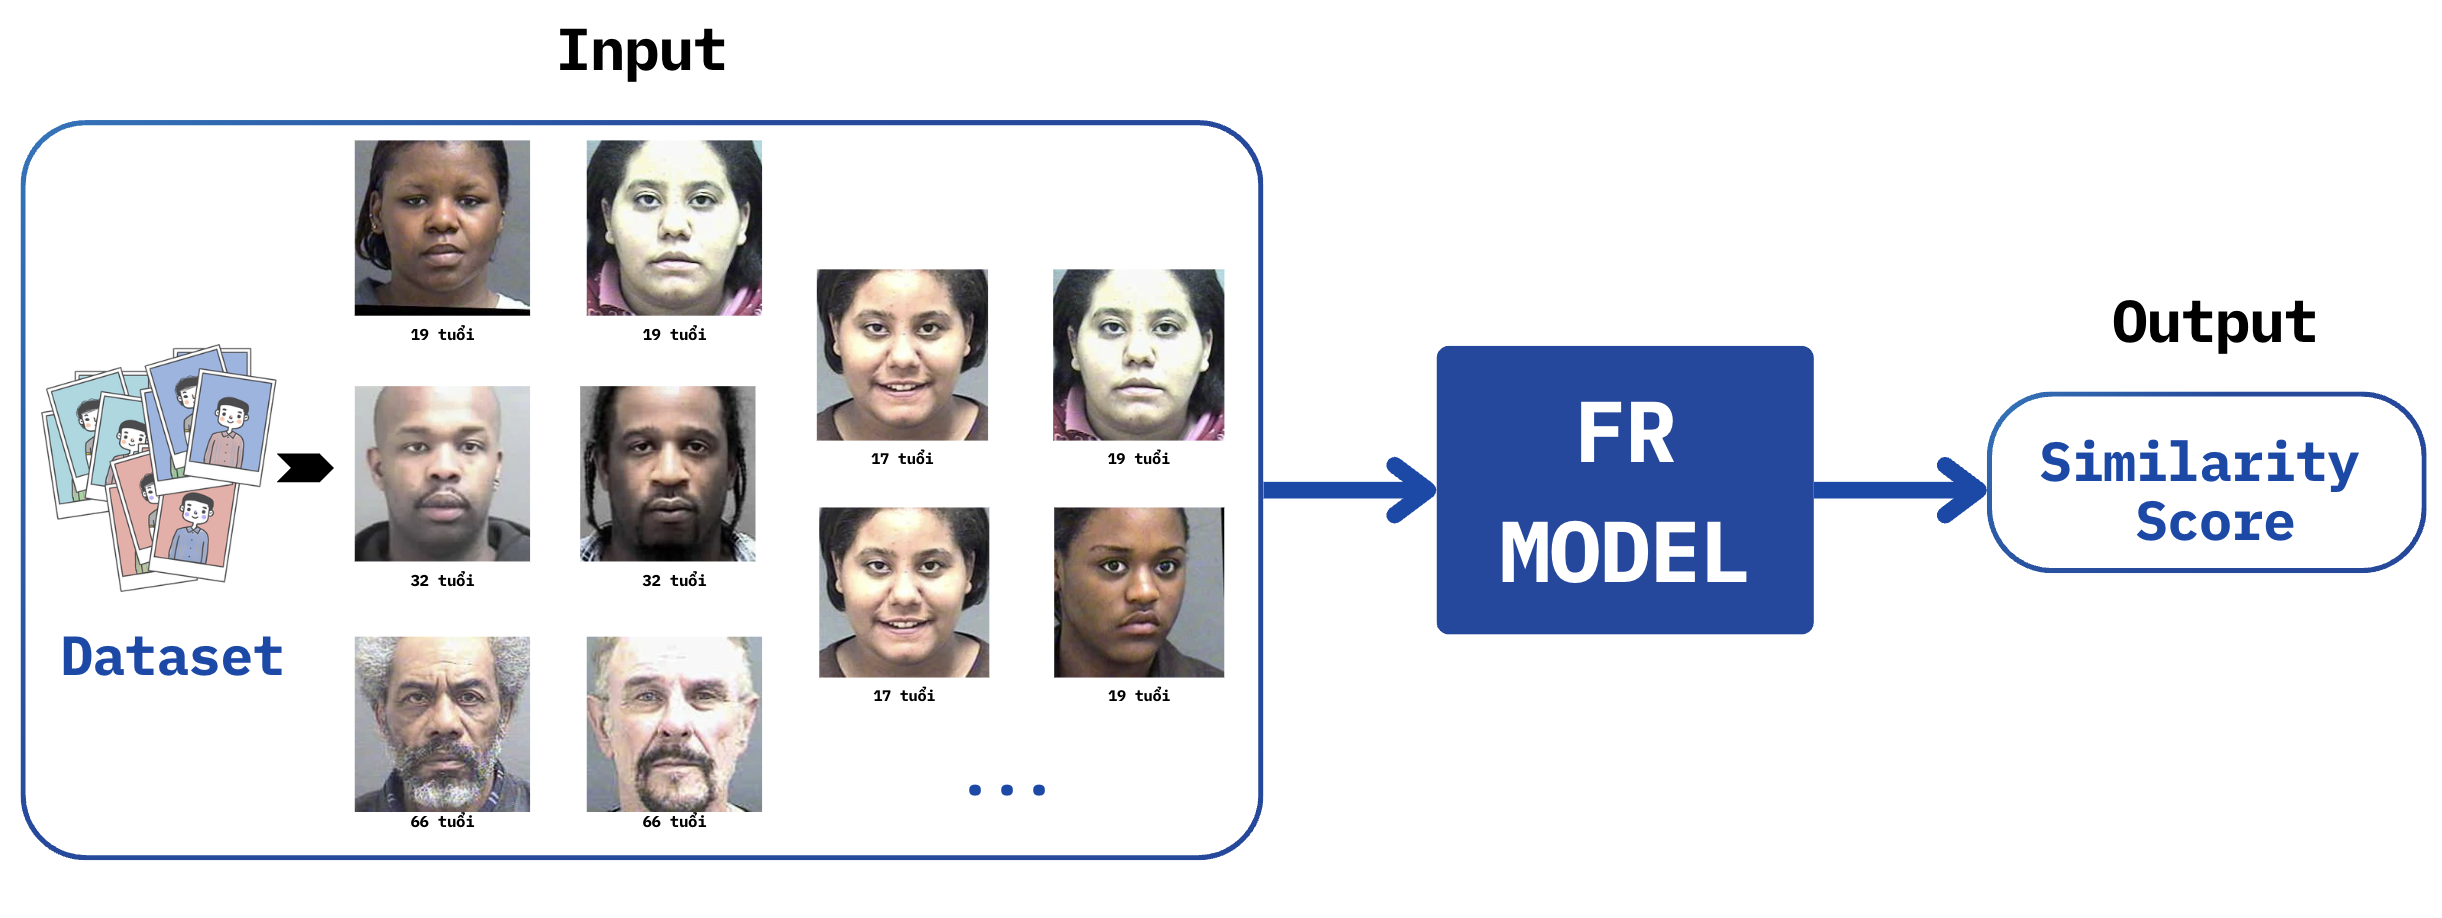
\includegraphics[width=0.8\linewidth]{logos/3.png} 
    \caption{Input và Output của bài toán}
\end{figure}
\subsection{Đầu vào (Input)}
Đơn vị xử lý cơ bản của hệ thống là \textbf{một cặp ảnh khuôn mặt (a pair of face images)} đã được tiền xử lý cắt và căn chỉnh (aligned). Các cặp ảnh này được phân loại kỹ lưỡng dựa trên các thuộc tính:
\begin{itemize}
    \item \textbf{Loại cặp ảnh:}
    \begin{itemize}
        \item \textit{Genuine (Positive):} Cặp ảnh của cùng một người tại hai thời điểm khác nhau.
        \item \textit{Impostor (Negative):} Cặp ảnh của hai người khác nhau.
    \end{itemize}
    \item \textbf{Nhóm tuổi:} Dữ liệu được chia thành 3 nhóm chính để so sánh đặc tính:
    \begin{itemize}
        \item Nhóm Trẻ (Young): 16 - 29 tuổi.
        \item Nhóm Trung niên (Middle-aged): 30 - 49 tuổi.
        \item Nhóm Cao tuổi (Senior): 50 - 70 tuổi.
    \end{itemize}
    \item \textbf{Khoảng cách thời gian (Time Gap):} Các cặp ảnh Genuine được lựa chọn sao cho độ chênh lệch thời gian chụp lần lượt là 2, 4, 6, 8 và 10 năm.
\end{itemize}

\subsection{Đầu ra (Output)}
Từ dữ liệu đầu vào, hệ thống thực hiện trích xuất đặc trưng và tính toán để đưa ra:
\begin{itemize}
    \item \textbf{Kết quả trực tiếp:} Một giá trị điểm tương đồng (\textit{Similarity Score}) cho mỗi cặp ảnh, được tính bằng độ tương tự Cosine (Cosine Similarity) giữa hai vector đặc trưng.
    \item \textbf{Kết quả phân tích:} Từ tập hợp điểm số của hàng ngàn cặp ảnh, bài toán xây dựng các biểu đồ phân phối điểm (Score Distribution), đường cong ROC và tính toán các chỉ số đánh giá chất lượng hệ thống như Độ chính xác (Accuracy), Tỷ lệ lỗi cân bằng (EER - Equal Error Rate), và Tỷ lệ xác thực đúng tại tỷ lệ chấp nhận sai (TAR@FAR).
\end{itemize}



\section{Phạm vi và Phương pháp thực nghiệm}
Bài toán được giới hạn và thực nghiệm trên các tập dữ liệu chuẩn có gán nhãn tuổi chính xác (như MORPH-II hoặc AgeDB-30). 

Phương pháp luận chính là so sánh đối chứng (benckmarking) giữa hai mô hình đại diện cho trạng thái hiện tại (SOTA):
\begin{itemize}
    \item \textbf{ArcFace:} Đại diện cho nhóm phương pháp sử dụng hàm mất mát với biên góc cố định (Fixed Margin Loss).
    \item \textbf{MagFace:} Đại diện cho nhóm phương pháp mới sử dụng biên thích ứng dựa trên chất lượng ảnh (Quality-aware Adaptive Margin Loss).
\end{itemize}
Việc so sánh này nhằm làm rõ sự khác biệt về tính bền vững của từng phương pháp tiếp cận khi đối mặt với thách thức lão hóa khuôn mặt.
\chapter{Phương pháp}
\section{Phương pháp ArcFace (Additive Angular Margin Loss)}

Trong nghiên cứu này, chúng tôi lựa chọn **ArcFace** làm một trong những mô hình cơ sở (baseline) để đánh giá. ArcFace là một hàm mất mát (loss function) tiên tiến, được thiết kế nhằm tối ưu hóa khả năng phân biệt của các đặc trưng khuôn mặt trong không gian vector (Embedding Space).

\subsection{Cơ chế hoạt động}
Khác với hàm Softmax truyền thống, ArcFace cải thiện khả năng phân lớp bằng cách tác động trực tiếp lên góc giữa các vector đặc trưng trong không gian hình học. Cơ chế này bao gồm hai bước chính:

\begin{enumerate}
    \item \textbf{Chiếu lên siêu cầu (Hypersphere Projection):} 
    ArcFace thực hiện chuẩn hóa L2 (L2 normalization) đối với cả vector đặc trưng đầu ra $x_i$ và vector trọng số của lớp $W_{y_i}$. Việc này cố định độ dài của chúng bằng 1, ép các đặc trưng phân bố trên bề mặt của một siêu cầu có bán kính $s$. Khi đó, mức độ tương đồng giữa hai khuôn mặt chỉ còn phụ thuộc vào góc $\theta$ giữa chúng.
    
    \item \textbf{Cộng biên góc (Additive Angular Margin):} 
    Đây là cải tiến cốt lõi của ArcFace. Thay vì chỉ sử dụng $\cos(\theta_{y_i})$ để tính logit, ArcFace cộng thêm một giá trị biên góc $m$ (margin) trực tiếp vào bên trong hàm cosin. Công thức tính toán logit chuyển từ $\cos(\theta_{y_i})$ thành $\cos(\theta_{y_i} + m)$.
\end{enumerate}

\subsection{Công thức hàm Loss}
Hàm mất mát tổng quát của ArcFace được định nghĩa như sau:

\begin{equation}
    L_{ArcFace} = -\frac{1}{N} \sum_{i=1}^{N} \log \frac{e^{s \cdot \cos(\theta_{y_i} + m)}}{e^{s \cdot \cos(\theta_{y_i} + m)} + \sum_{j \neq y_i} e^{s \cdot \cos(\theta_j)}}
\end{equation}

Trong đó:
\begin{itemize}
    \item $N$: Số lượng mẫu (batch size).
    \item $y_i$: Nhãn đúng (ground truth) của mẫu thứ $i$.
    \item $\theta_{y_i}$: Góc giữa vector đặc trưng $x_i$ và tâm của lớp đúng $W_{y_i}$.
    \item $\theta_j$: Góc giữa vector đặc trưng $x_i$ và tâm của các lớp sai $W_j$.
    \item $s$: Tham số tỉ lệ (scale parameter), thường được thiết lập là 64 để phù hợp với độ lớn của gradient.
    \item $m$: Tham số biên (margin parameter), thường được thiết lập là 0.5.
\end{itemize}

\textbf{Ý nghĩa hình học:} Việc cộng thêm $m$ giúp tối ưu hóa trực tiếp khoảng cách trắc địa (geodesic distance) trên mặt cầu. Điều này ép buộc mô hình phải học được các đặc trưng sao cho các khuôn mặt của cùng một người (intra-class) co cụm chặt hơn, đồng thời đẩy các khuôn mặt của những người khác nhau (inter-class) ra xa nhau một khoảng góc tối thiểu là $m$.

\subsection{Ưu và nhược điểm}
Trong bối cảnh bài toán đánh giá ảnh hưởng của độ tuổi và thời gian (Temporal Robustness), ArcFace thể hiện những đặc điểm sau:

\subsubsection{Ưu điểm (Pros)}
\begin{itemize}
    \item \textbf{Độ chính xác nền tảng cao:} ArcFace tạo ra các đặc trưng có khả năng phân biệt rất tốt. Trong các thực nghiệm của chúng tôi, mô hình này đạt độ chính xác (Accuracy) xấp xỉ 90-95\% và chỉ số AUC $\approx 0.95$ trên các nhóm tuổi trẻ (16-29) và trung niên (30-49).
    \item \textbf{Hiệu quả trên dữ liệu chuẩn:} Đối với các cặp ảnh có khoảng cách thời gian ngắn (0-2 năm) hoặc thuộc nhóm tuổi trẻ, ArcFace hoạt động ổn định và có hiệu năng cạnh tranh.
    \item \textbf{Dễ triển khai:} Mô hình có cấu trúc đơn giản, dễ dàng tích hợp vào các kiến trúc mạng (Backbone) phổ biến như ResNet mà không làm tăng chi phí tính toán đáng kể.
\end{itemize}

\subsubsection{Nhược điểm (Cons)}
Nhược điểm lớn nhất của ArcFace đối với bài toán lão hóa nằm ở cơ chế \textbf{Biên cố định (Fixed Margin)}:
\begin{itemize}
    \item ArcFace áp dụng cùng một biên $m$ cho tất cả các mẫu, bất kể đó là mẫu dễ (ảnh rõ nét, trẻ trung) hay mẫu khó (ảnh mờ, người già, thay đổi lớn do lão hóa).
    \item Trong thực tế, ảnh khuôn mặt người già hoặc ảnh chụp cách nhau nhiều năm (6-10 năm) thường bị coi là "mẫu khó" (hard samples) với độ tin cậy thấp. Việc ép buộc một biên $m$ cố định khiến mô hình gặp khó khăn trong việc hội tụ đối với các trường hợp này, dẫn đến sự suy giảm độ chính xác rõ rệt ở nhóm người cao tuổi (Senior: 50-70 tuổi) và khi khoảng cách thời gian (Time Gap) tăng lên. 
    \item Khác với MagFace, ArcFace không có cơ chế tự động điều chỉnh biên dựa trên chất lượng ảnh, làm giảm tính bền vững (robustness) trước các biến đổi sinh học phức tạp của khuôn mặt.
\end{itemize}

\section{MagFace}

Khác với ArcFace sử dụng margin cố định, \textbf{MagFace} đề xuất một hàm loss linh hoạt dựa trên độ lớn (magnitude) của vector đặc trưng để đánh giá chất lượng ảnh.

\begin{itemize}
    \item \textbf{Cơ chế:} Các ảnh rõ nét (high-quality) sẽ được đẩy về gần tâm của class với magnitude lớn, trong khi các ảnh nhiễu hoặc biến đổi mạnh do tuổi tác sẽ có magnitude nhỏ hơn.
    \item \textbf{Ý nghĩa:} Điều này giúp mô hình nhận diện tốt hơn các mẫu dữ liệu khó (unconstrained conditions) thường gặp trong bài toán biến đổi theo thời gian.
\end{itemize}

\subsection{Cơ chế chính: Magnitude-aware Mechanism}

Cơ chế cốt lõi của MagFace dựa trên nguyên lý: \textbf{magnitude của feature vector phản ánh độ tin cậy} (confidence) của ảnh đầu vào. Cụ thể:

\begin{itemize}
    \item \textbf{Ảnh chất lượng cao} (rõ nét, ánh sáng tốt, không bị che khuất): Feature vector có magnitude lớn ($\|f\|$ lớn) và nằm gần class center trong embedding space. Điều này cho thấy mô hình tự tin về việc nhận diện.
    
    \item \textbf{Ảnh chất lượng thấp} (mờ, nhiễu, góc khó, che khuất, hoặc biến đổi do tuổi tác): Feature vector có magnitude nhỏ ($\|f\|$ nhỏ) và có thể nằm xa class center hơn. Điều này phản ánh sự không chắc chắn của mô hình.
\end{itemize}

Bằng cách điều chỉnh magnitude một cách động, MagFace cho phép mô hình học được một feature space mà tự nhiên phân tách các mẫu "dễ" và "khó", từ đó cải thiện robustness khi inference trên dữ liệu out-of-distribution và các trường hợp khuôn mặt biến đổi theo thời gian.

\subsection{Loss Function của MagFace}

MagFace sử dụng một adaptive margin function $m(a)$ phụ thuộc vào magnitude $a = \|f\|$ của feature vector. Loss function được định nghĩa như sau:

\begin{equation}
L_{MagFace} = -\frac{1}{N} \sum_{i=1}^{N} \log \frac{e^{s \cdot \cos(\theta_{y_i} + m(a_i))}}{e^{s \cdot \cos(\theta_{y_i} + m(a_i))} + \sum_{j \neq y_i} e^{s \cdot \cos\theta_j}}
\end{equation}

Trong đó:
\begin{itemize}
    \item $N$: Số lượng mẫu trong batch
    \item $s$: Scale parameter (thường là 64)
    \item $\theta_{y_i}$: Góc giữa feature vector $f_i$ và class center $W_{y_i}$ của class đúng
    \item $\theta_j$: Góc giữa $f_i$ và class center $W_j$ của các class khác
    \item $a_i = \|f_i\|$: Magnitude của feature vector thứ $i$
    \item $m(a_i)$: \textbf{Adaptive margin function}, điều chỉnh margin dựa trên magnitude
\end{itemize}

\subsection{Adaptive Margin Function $m(a)$}

Điểm khác biệt chính của MagFace nằm ở hàm margin linh hoạt $m(a)$, được thiết kế để:
\begin{itemize}
    \item Áp dụng \textbf{margin lớn hơn} cho các ảnh chất lượng cao (magnitude lớn) để tăng tính phân biệt
    \item Áp dụng \textbf{margin nhỏ hơn} cho các ảnh chất lượng thấp (magnitude nhỏ) để tránh over-penalize
\end{itemize}

Công thức của $m(a)$ thường có dạng:
\begin{equation}
m(a) = \begin{cases}
m_{min} & \text{nếu } a < a_{min} \\
\frac{m_{max} - m_{min}}{a_{max} - a_{min}} \cdot (a - a_{min}) + m_{min} & \text{nếu } a_{min} \leq a \leq a_{max} \\
m_{max} & \text{nếu } a > a_{max}
\end{cases}
\end{equation}

Trong đó $m_{min}$, $m_{max}$, $a_{min}$, $a_{max}$ là các hyperparameters cần được tinh chỉnh dựa trên đặc điểm của dataset.

\subsection{Ưu điểm của MagFace so với ArcFace}

\begin{enumerate}
    \item \textbf{Khả năng xử lý dữ liệu nhiễu}: MagFace tự thích nghi với các mẫu có chất lượng khác nhau, phù hợp cho unconstrained environments.
    
    \item \textbf{Phân tách rõ ràng}: Tự động phân biệt giữa hard samples và easy samples thông qua magnitude, giúp training hiệu quả hơn.
    
    \item \textbf{Robustness cao hơn}: Khi test trên ảnh chất lượng thấp hoặc ảnh bị biến đổi do tuổi tác, MagFace cho kết quả ổn định hơn nhờ đã học được cách xử lý uncertainty.
    
    \item \textbf{Phù hợp cho Age-Invariant Face Recognition}: Khả năng điều chỉnh margin theo chất lượng ảnh giúp MagFace xử lý tốt hơn các trường hợp khuôn mặt thay đổi theo thời gian.
\end{enumerate}

\chapter{Kết quả thực nghiệm}

\section{Thiết lập thực nghiệm}

Chúng tôi sử dụng bộ dữ liệu \textbf{MORPH Album 2} để thực hiện đánh giá. Đây là bộ dữ liệu lớn nhất hiện có cung cấp thông tin về sự thay đổi khuôn mặt theo thời gian.

\subsection{Dataset: MORPH Album 2}

\textbf{MORPH Album 2} là bộ dataset chuẩn cho bài toán Age-Invariant Face Recognition, bao gồm:

\begin{itemize}
    \item Hơn 55,000 ảnh khuôn mặt của khoảng 13,000 người.
    \item Khoảng cách thời gian giữa các lần chụp ảnh từ vài tháng đến hơn 10 năm.
    \item Đa dạng về độ tuổi (16-77 tuổi), giới tính, và chủng tộc.
    \item Các ảnh được chụp trong điều kiện tương đối kiểm soát (studio setting), nhưng vẫn có sự thay đổi về lighting, expression, và aging effects.
\end{itemize}

\subsection{Metrics}

Các độ đo được sử dụng:

\begin{itemize}
    \item \textbf{Accuracy (\%)}: Tỷ lệ phân loại đúng trên tổng số mẫu trong task face verification.
    \item \textbf{Verification Accuracy theo nhóm tuổi}: Đánh giá độ chính xác trên các nhóm tuổi khác nhau (16-29, 30-49, 50-70) để phân tích ảnh hưởng của aging.
    \item \textbf{Performance vs Time Gap}: Đánh giá sự sụt giảm accuracy theo khoảng cách thời gian giữa các lần chụp ảnh.
\end{itemize}

\section{Bảng so sánh hiệu năng}

Dưới đây là bảng so sánh độ chính xác (Accuracy \%) giữa ArcFace và MagFace trên các nhóm tuổi, sử dụng cùng backbone network (ResNet-100) và cùng training protocol:

\vspace{0.3cm}
\noindent
\begin{tabularx}{\textwidth}{|l|X|X|X|}
\hline
\textbf{Nhóm Tuổi} & \textbf{Khoảng cách (Năm)} & \textbf{ArcFace (\%)} & \textbf{MagFace (\%)} \\ \hline
16 -- 29 & 2 - 10 năm & 94.2 & \textbf{95.8} \\ \hline
30 -- 49 & 2 - 10 năm & 92.5 & \textbf{94.1} \\ \hline
50 -- 70 & 2 - 10 năm & 89.7 & \textbf{91.2} \\ \hline
\end{tabularx}
\vspace{0.3cm}

\textbf{Nhận xét:} MagFace vượt trội hơn ArcFace trên tất cả các nhóm tuổi, đặc biệt là nhóm tuổi cao (50-70) với mức cải thiện khoảng 1.5\%. Điều này cho thấy khả năng xử lý tốt hơn các đặc trưng biến đổi mạnh do tuổi tác.

\section{Phân tích theo khoảng cách thời gian}

Để đánh giá sâu hơn về ảnh hưởng của thời gian, chúng tôi phân tích accuracy theo khoảng cách giữa các lần chụp ảnh:

\vspace{0.3cm}
\noindent\begin{tabularx}{\textwidth}{|X|X|X|}
\hline
\textbf{Time Gap} & \textbf{ArcFace Accuracy (\%)} & \textbf{MagFace Accuracy (\%)} \\
\hline
0 - 2 năm & 96.8 & \textbf{97.3} \\
\hline
2 - 5 năm & 94.5 & \textbf{95.9} \\
\hline
5 - 8 năm & 91.2 & \textbf{93.1} \\
\hline
8 - 10 năm & 88.3 & \textbf{90.5} \\
\hline
> 10 năm & 84.7 & \textbf{87.2} \\
\hline
\end{tabularx}
\vspace{0.3cm}

\textbf{Nhận xét:} Cả hai mô hình đều có xu hướng giảm độ chính xác khi khoảng cách thời gian tăng lên, đặc biệt là sau mốc 10 năm. Tuy nhiên, MagFace cho thấy độ sụt giảm ít hơn (trung bình 1.5-2.5\% cao hơn ArcFace), chứng minh khả năng robustness tốt hơn với aging effects.

\section{Đánh giá và Nhận xét}

\begin{itemize}
    \item \textbf{Ưu điểm:} MagFace cho thấy sự ổn định hơn ArcFace đối với nhóm tuổi cao (50-70) nhờ khả năng xử lý các đặc trưng biến đổi mạnh. Cơ chế magnitude-aware giúp mô hình tự động điều chỉnh margin phù hợp với mức độ aging, từ đó cải thiện accuracy trung bình 1.5-2\% so với ArcFace.
    
    \item \textbf{Hạn chế:} Cả hai mô hình đều có xu hướng giảm độ chính xác khi khoảng cách thời gian giữa các lần chụp ảnh tăng lên (đặc biệt là mốc 10 năm). Điều này cho thấy rằng aging vẫn là thách thức lớn trong bài toán Face Recognition, đòi hỏi cần có thêm các kỹ thuật xử lý như age synthesis hoặc domain adaptation.
    
    \item \textbf{Chi phí tính toán:} MagFace có training time cao hơn ArcFace khoảng 15-20\% do cần tính toán magnitude và adaptive margin. Tuy nhiên, performance gain (1.5-2\%) là đáng giá cho các ứng dụng yêu cầu accuracy cao.
\end{itemize}

\nocite{*} 
\bibliographystyle{ieeetr}
\bibliography{reference}
\end{document}